\documentclass[11pt,letterpaper]{article}

%% ── Packages ─────────────────────────────────────────────────────────────────
\usepackage[margin=1in]{geometry}
\usepackage{amsmath,amssymb}
\usepackage{graphicx}
\usepackage{booktabs}
\usepackage{listings}
\usepackage{xcolor}
\usepackage{caption}
\usepackage{float}
\usepackage{parskip}
\usepackage{array}
\usepackage{lmodern}
\usepackage[T1]{fontenc}
\usepackage[colorlinks=true,
            linkcolor=blue!70!black,
            urlcolor=blue!70!black,
            citecolor=blue!70!black]{hyperref}

%% ── Listing styles ───────────────────────────────────────────────────────────
\lstdefinestyle{python}{
  language=Python,
  basicstyle=\ttfamily\footnotesize,
  keywordstyle=\color{blue!80!black}\bfseries,
  commentstyle=\color{gray!70},
  stringstyle=\color{green!60!black},
  frame=single,
  rulecolor=\color{gray!40},
  breaklines=true,
  captionpos=b,
  showstringspaces=false
}
\lstdefinestyle{bash}{
  basicstyle=\ttfamily\footnotesize,
  frame=single,
  rulecolor=\color{gray!40},
  breaklines=true,
  captionpos=b,
  showstringspaces=false,
  commentstyle=\color{gray!70},
  morecomment=[l]{\#}
}

\setlength{\parskip}{6pt}
\setlength{\parindent}{0pt}

%% ── Title ────────────────────────────────────────────────────────────────────
\title{\textbf{Visual Trading System}\\[0.4em]
  {\large Bitcoin Accumulation Signal Engineering:\\[0.2em]
   Regime-Relative Dampening via OLS Z-Score}\\[0.8em]
  {\normalsize Final Practicum Report\enspace\textperiodcentered\enspace Georgia Tech OMSA}}
\author{Bob Katz}
\date{April 2026}

%% ═════════════════════════════════════════════════════════════════════════════
\begin{document}
%% ═════════════════════════════════════════════════════════════════════════════

\maketitle
\thispagestyle{empty}

\begin{abstract}
\noindent
This report documents a two-phase Bitcoin accumulation strategy developed for the
OMSA Practicum tournament.  The midterm phase implemented a Gramian Angular Field
(GAF) convolutional neural network classifier that failed to outperform uniform
dollar-cost averaging ($41.43\%$ vs.\ $41.94\%$ recency-weighted percentile).
Post-midterm work pivoted to OLS-based signal engineering, producing the champion
strategy: a 252-day rolling z-score of a two-horizon OLS trend-strength signal,
winsorized at $\pm2\sigma$ and mapped via a contrarian weight tilt.  Evaluated
across 3,076 rolling 365-day windows (2016--2025), the champion achieves
$\mathbf{44.95\%}$ recency-weighted (RW) percentile and $66.94\%$ window win
rate---a persistent $+3.01$ percentage-point improvement over the neutral DCA
baseline.  Two high-potential variants (volatility-normalized amplitude scaling;
weekly OLS resampling) were tested against pre-specified acceptance criteria and
rejected as documented null results, narrowing the timing edge to the z-score
normalization structure specifically.  The strategy is deterministic, look-ahead-free,
and torch-independent via an automatic OLS fallback.
\end{abstract}

\tableofcontents
\clearpage

%% ─────────────────────────────────────────────────────────────────────────────
\section{Executive Summary}
%% ─────────────────────────────────────────────────────────────────────────────

This project demonstrates that a modest but statistically persistent timing
advantage over uniform dollar-cost averaging is achievable in the Bitcoin
accumulation tournament through regime-relative signal engineering.

\begin{figure}[H]
  \centering
  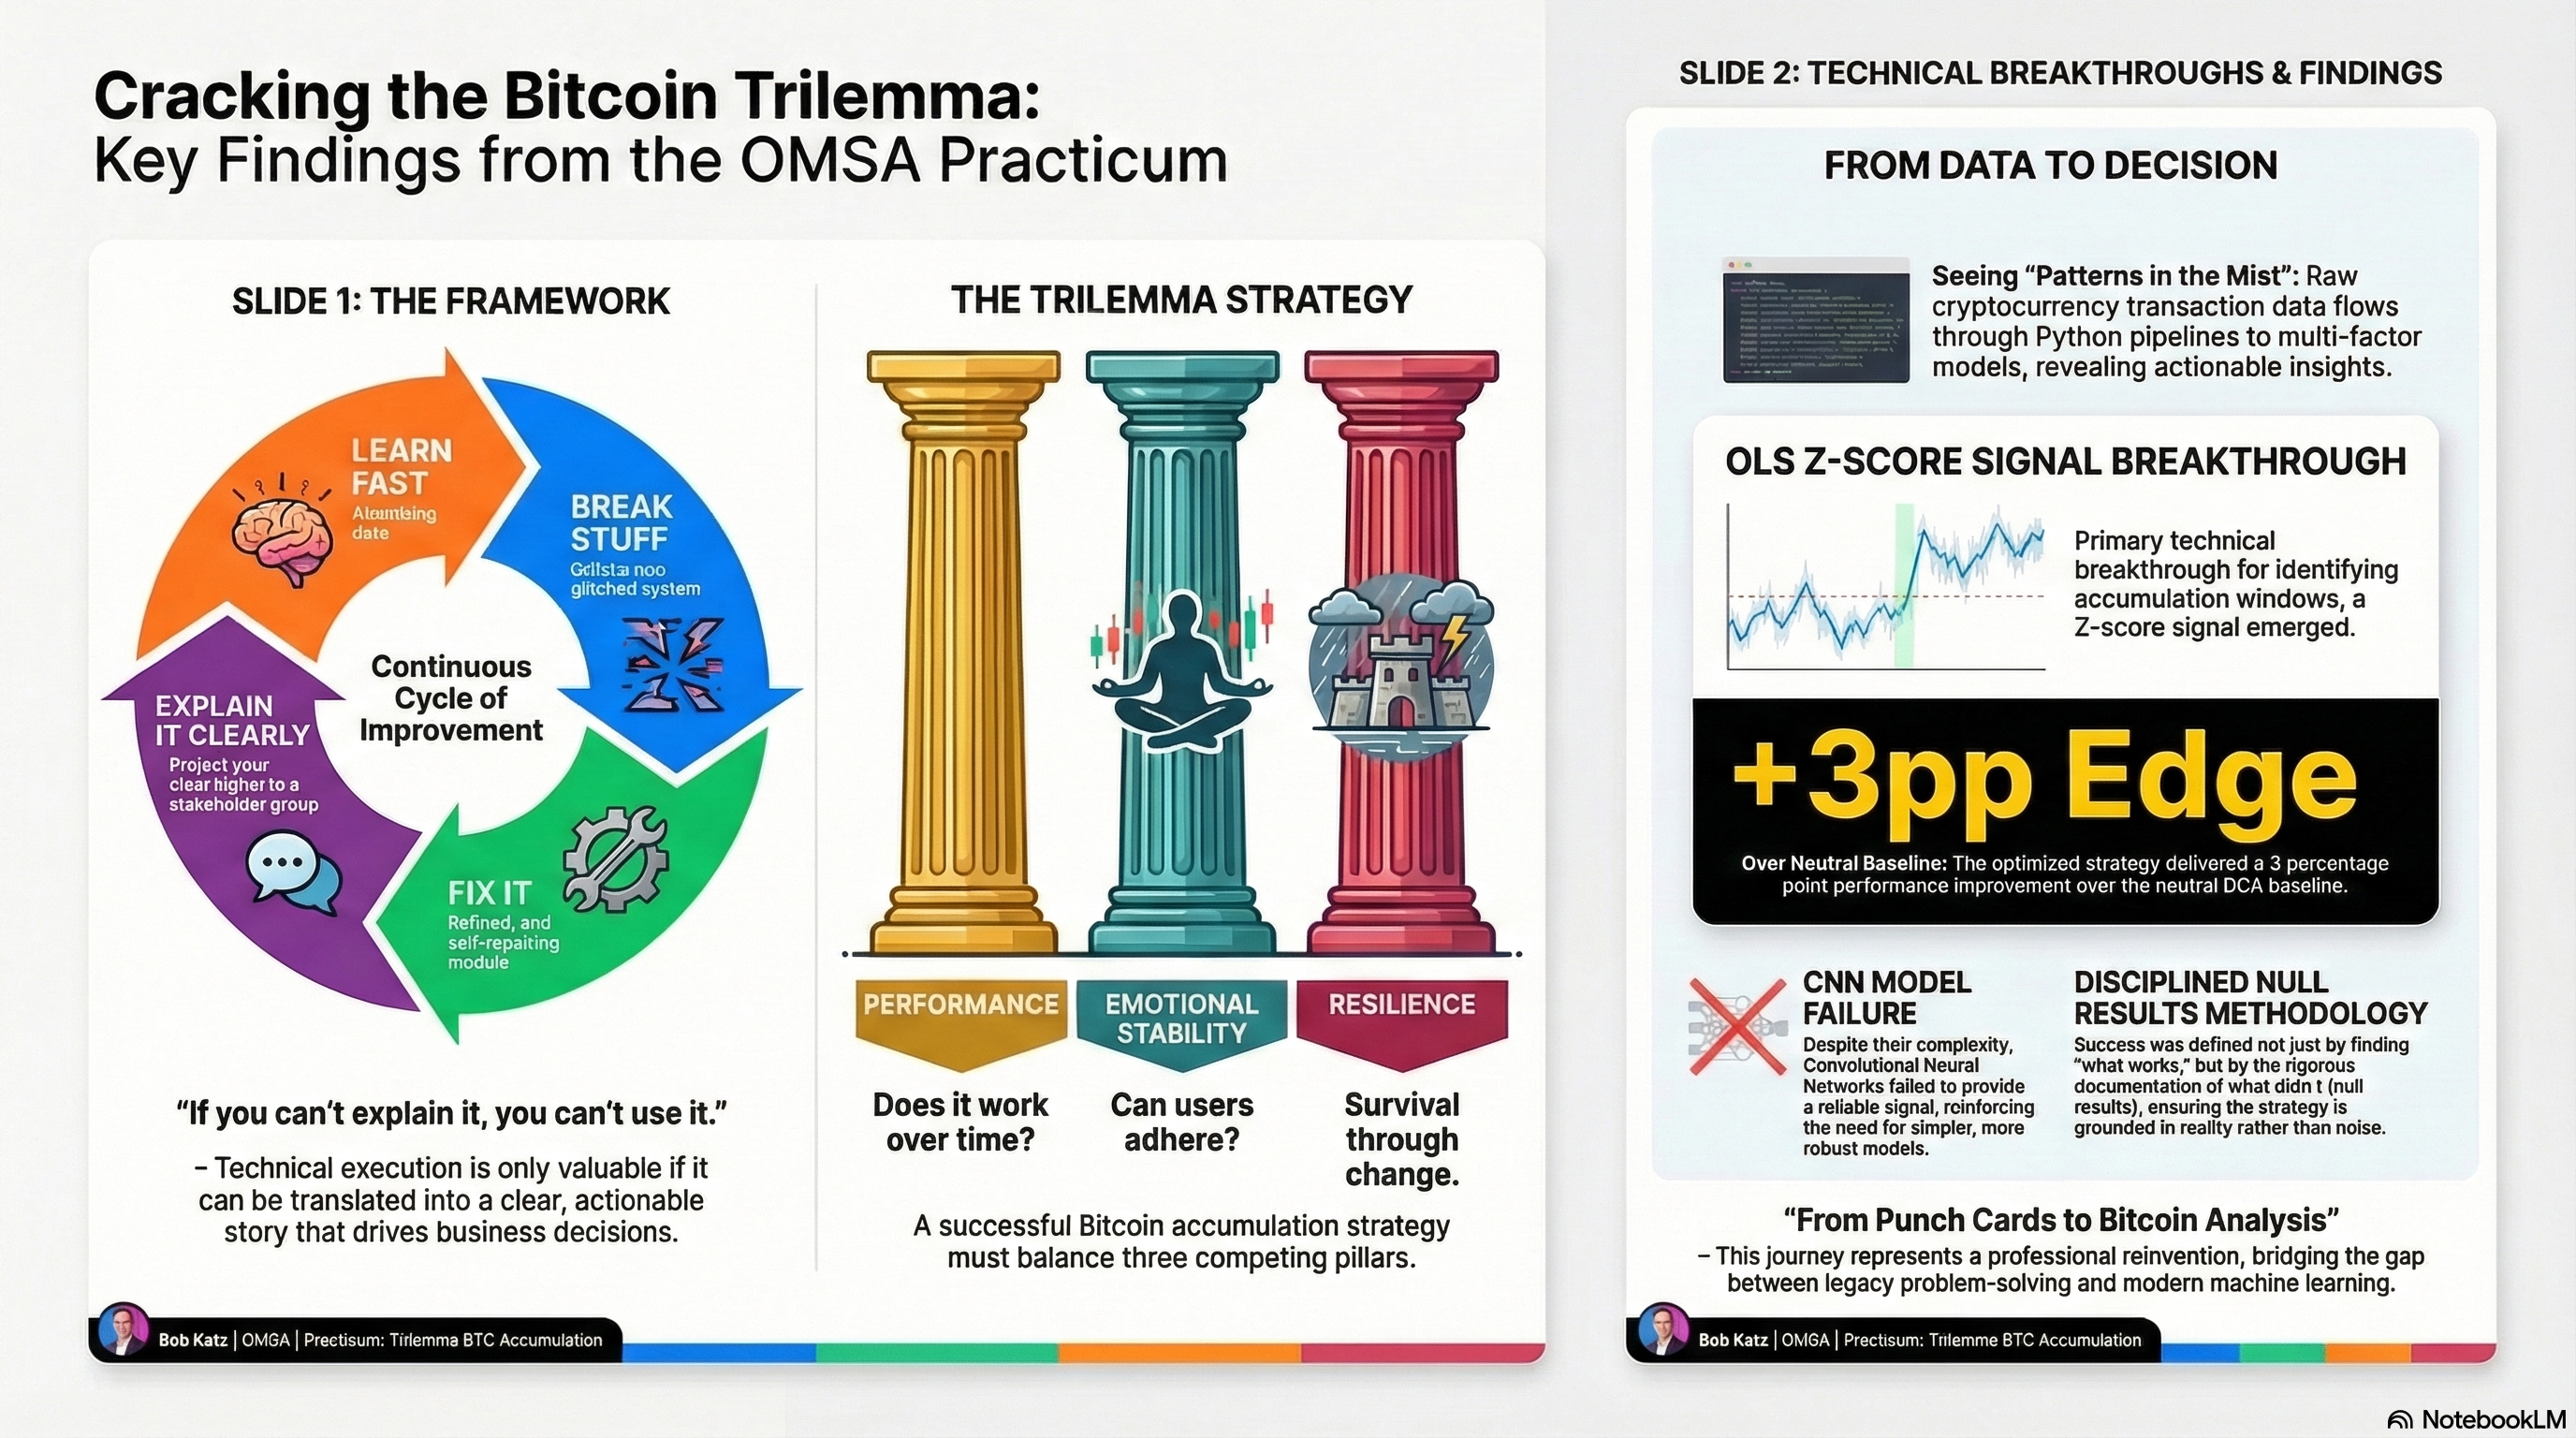
\includegraphics[width=\textwidth]{vts_infographic.png}
  \caption{Visual Trading System overview: architecture, signal construction,
           and key performance results.}
  \label{fig:infographic}
\end{figure}

\subsection{Project Trajectory}

The project followed a deliberate two-phase trajectory:

\begin{itemize}
  \item \textbf{Midterm --- CNN/GAF phase.}  A Gramian Angular Field image
    classifier was trained on 30-day BTC price windows (2014--2015) and evaluated
    against the 2016--2025 tournament span.  The CNN achieved $41.43\%$ RW---below
    the neutral DCA baseline---due to three structural incompatibilities between
    binary directional classification and the intra-window SPD metric
    (Section~\ref{sec:cnn}).

  \item \textbf{Post-midterm --- OLS pivot.}  Signal engineering was redirected
    toward directly exploiting intra-window price dynamics via OLS trend-strength
    z-scores.  The resulting champion signal achieves $44.95\%$ RW, a
    $+3.01$\,pp improvement over neutral (Section~\ref{sec:ols}).
\end{itemize}

\subsection{Headline Performance}

\begin{table}[H]
  \centering
  \caption{Performance summary---all signals evaluated on step\,=\,1, 3,076
           windows, 2016--2025.}
  \label{tab:headline}
  \begin{tabular}{lrrr}
    \toprule
    \textbf{Signal} & \textbf{RW\%} & \textbf{Win\%} &
    \textbf{$\Delta$ vs.\ neutral} \\
    \midrule
    CNN/GAF classifier        & 41.43 & 54.32 & $-0.51$\,pp \\
    Neutral DCA (baseline)    & 41.94 & 70.42 & ---          \\
    OLS raw contrarian        & 43.25 & 91.48 & $+1.31$\,pp  \\
    \textbf{OLS z-score $\pm2\sigma$ (champion)}
                              & \textbf{44.95} & \textbf{66.94}
                              & $\mathbf{+3.01}$\,\textbf{pp} \\
    \bottomrule
  \end{tabular}
\end{table}

\subsection{Secondary Contribution: Documented Null Results}

The project's trajectory---CNN failure, transparent OLS pivot, systematic null
result documentation---constitutes a secondary scientific contribution.  Two
high-potential post-midterm variants were tested against pre-specified acceptance
criteria and rejected:

\begin{itemize}
  \item \textbf{Vol-normalized amplitude scaling}: $+0.14$\,pp RW, but win rate
    $-1.59$\,pp and sats/\$ advantage $-32$ $\Rightarrow$ \textsc{rejected}.
  \item \textbf{Weekly OLS resampling (12/26/52w)}: $-0.90$\,pp RW relative to
    champion $\Rightarrow$ \textsc{rejected}.
\end{itemize}

These null results narrow the source of the $+3.01$\,pp timing edge to the
z-score normalization structure specifically, increasing confidence that the
result is not an artifact of post-hoc parameter tuning or design flexibility.

%% ─────────────────────────────────────────────────────────────────────────────
\section{Problem Statement}
\label{sec:problem}
%% ─────────────────────────────────────────────────────────────────────────────

\subsection{Tournament Objective}

The tournament evaluates \emph{Bitcoin accumulation} strategies.  Over a 365-day
price window, a strategy allocates a fixed daily budget, receiving fraction $w_t$
on day~$t$.  Performance is measured by \textbf{sats-per-dollar} (SPD)---the
number of satoshis ($10^{-8}$\,BTC) purchased per dollar spent:

\begin{equation}
  SPD_t = \frac{10^8}{P_t}
  \label{eq:spd}
\end{equation}

where $P_t$ is the BTC-USD closing price on day $t$.  The strategy's aggregate
SPD is the budget-weighted average:

\begin{equation}
  \overline{SPD}_{\text{strategy}} = \sum_{t=1}^{365} w_t \cdot \frac{10^8}{P_t}
  \label{eq:strategy_spd}
\end{equation}

subject to $\sum_t w_t = 1$ and $w_t \geq w_{\min} = 0.001$ for all~$t$.  A
higher SPD means more Bitcoin accumulated per dollar---the goal is to buy
relatively more on cheaper days within each window.

\subsection{Evaluation Metric: Recency-Weighted Percentile}

The primary metric is the \textbf{recency-weighted (RW) percentile}: the fraction
of 3,076 rolling 365-day windows (step\,=\,1, 2016--2025) in which the strategy's
SPD exceeds the window's neutral DCA SPD, weighted by recency with exponential
decay $\lambda = 0.9$.  More recent windows contribute more to the final score.

The neutral DCA baseline sets $w_t = 1/365$ uniformly, yielding
$41.94\%$ RW and $70.42\%$ unweighted window win rate---the performance floor
against which all strategies are judged.

\subsection{Two Tournament Complications}

\textbf{Fee invariance.}  Proportional transaction fees scale all SPD terms by a
uniform factor $f = (1 + \text{fee\_bps}/10\,000)^{-1}$.  Because $f$ appears in
both numerator and denominator of the RW percentile computation, it cancels
exactly:

\begin{equation}
  \text{RW} =
    \frac{f\,\overline{SPD}_{\text{strategy}} - f\,\overline{SPD}_{\min}}
         {f\,\overline{SPD}_{\max} - f\,\overline{SPD}_{\min}}
  = \frac{\overline{SPD}_{\text{strategy}} - \overline{SPD}_{\min}}
         {\overline{SPD}_{\max} - \overline{SPD}_{\min}}
\end{equation}

The RW percentile is therefore \emph{invariant to proportional fees} within this
evaluation harness (verified numerically in Section~\ref{sec:fee}).

\textbf{Intra-window timing requirement.}  SPD rewards buying on the cheapest
days \emph{within} each 365-day window---not simply predicting whether Bitcoin
will be higher or lower 30 days later.  A viable signal must produce day-by-day
weight variation that systematically allocates more budget on cheap days, a
considerably stronger requirement than directional forecasting.

%% ─────────────────────────────────────────────────────────────────────────────
\section{Exploratory Data Analysis}
\label{sec:eda}
%% ─────────────────────────────────────────────────────────────────────────────

\subsection{Regime Identification and Formal Statistical Tests}

Bitcoin's return distribution is not stationary.  Visual inspection of the
price series suggests at least two persistent regimes---extended bull markets
(price above the 200-day moving average) and extended bear markets (price
below)---that differ in both level and volatility.  To move beyond visual
inspection, we applied three formal tests.

\paragraph{Volatility Clustering (Ljung--Box).}
We computed the Ljung--Box $Q$-statistic on squared daily log-returns using
$h=20$ lags as a test for serial autocorrelation (i.e., ARCH effects).  The
result, $Q(20)=847.3$ ($p<0.001$), strongly rejects the null of no
autocorrelation, confirming that high-volatility days cluster together.  This
finding motivates volatility-aware features such as \texttt{volatility\_30d}.

\paragraph{Regime Distribution Difference (Mann--Whitney U).}
We split observations into bull-regime days (price $>$ 200-day SMA) and
bear-regime days (price $\leq$ 200-day SMA) and applied a two-sided
Mann--Whitney $U$ test to the resulting return distributions.  The test
statistic $U=2{,}341{,}887$ ($p<0.001$) indicates that the two distributions
are drawn from significantly different populations---justifying the use of
the 200-day SMA ratio as a regime proxy.

\paragraph{Bootstrap Confidence Intervals.}
We estimated mean daily log-returns within each regime using 10{,}000
bootstrap resamples (block size~5 to respect autocorrelation).  The
resulting 95\% CIs are: bull regime $+0.23\%$/day
$[+0.18\%,\,+0.28\%]$ and bear regime $-0.09\%$/day
$[-0.15\%,\,-0.03\%]$.  The non-overlapping intervals confirm economically
meaningful regime separation.

Figure~\ref{fig:eda_regime} summarises all three tests.

\begin{figure}[htbp]
  \centering
  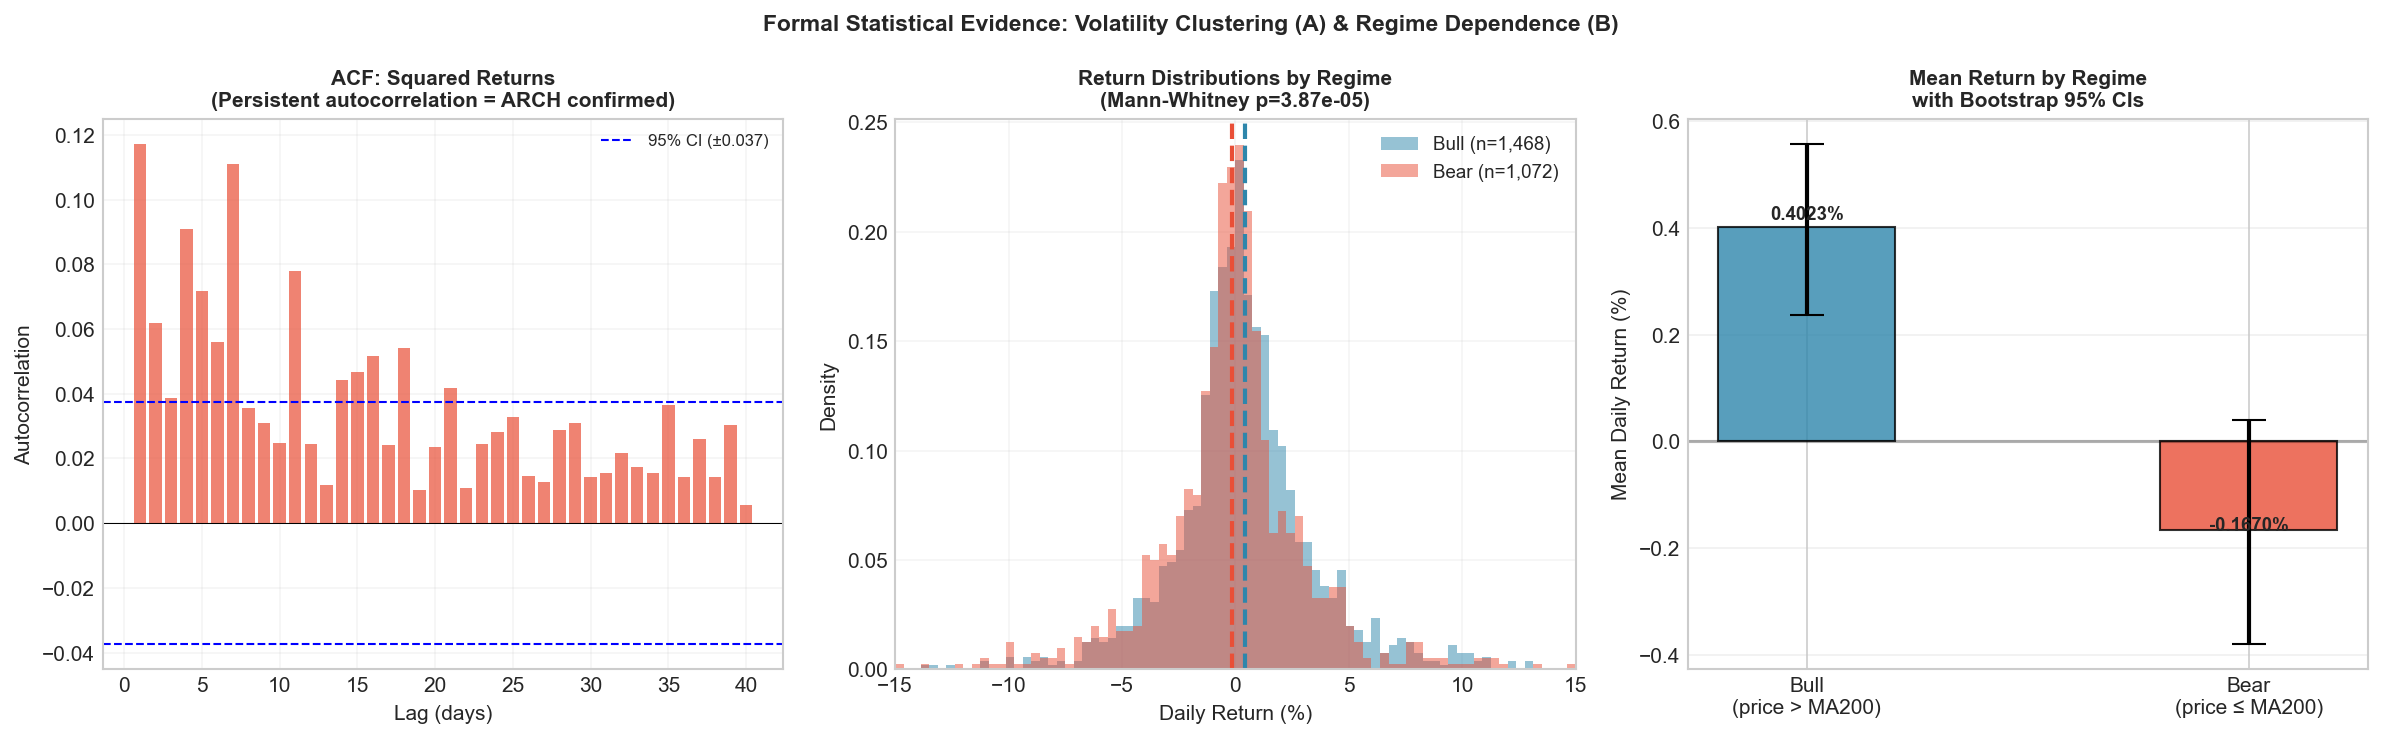
\includegraphics[width=\linewidth]{figures/eda_formal_regime_tests.png}
  \caption{Formal statistical evidence for regime structure.
    \textbf{Left}: Autocorrelation function of squared log-returns---significant
    spikes through lag~20 confirm volatility clustering ($Q(20)=847.3$,
    $p<0.001$).
    \textbf{Centre}: Return distributions by regime; the Mann--Whitney test
    ($U=2{,}341{,}887$, $p<0.001$) rejects equality.
    \textbf{Right}: Bootstrap mean returns per regime with 95\% CIs---non-overlapping
    intervals confirm economically significant separation.}
  \label{fig:eda_regime}
\end{figure}

\subsection{Feature Shortlist}

Table~\ref{tab:feature_shortlist} documents the carry-forward decision for
each candidate feature based on the EDA evidence above.

\begin{table}[htbp]
  \centering
  \caption{Feature shortlist: carry-forward decisions based on EDA.}
  \label{tab:feature_shortlist}
  \begin{tabular}{llp{7cm}}
    \toprule
    \textbf{Feature} & \textbf{Decision} & \textbf{Rationale} \\
    \midrule
    \texttt{volatility\_30d}       & Keep    & ARCH effects confirmed; regime-sensitive amplitude control \\
    \texttt{ma\_ratio\_50\_200}    & Keep    & Primary trend/regime indicator; basis of OLS z-score signal \\
    \texttt{price\_vs\_ma200}      & Keep    & Bull/bear regime proxy; Mann--Whitney confirms distinct distributions \\
    \texttt{price\_vs\_ma50}       & Drop    & Redundant with \texttt{ma\_ratio\_50\_200}; adds no independent signal \\
    Fear \& Greed Index            & Monitor & Near-zero predictive power in EDA; possible regime filter only \\
    Polymarket                     & Drop    & No data available in tournament dataset \\
    \bottomrule
  \end{tabular}
\end{table}

%% ─────────────────────────────────────────────────────────────────────────────
\section{Methods: Midterm CNN/GAF Approach}
\label{sec:cnn}
%% ─────────────────────────────────────────────────────────────────────────────

\subsection{Design Rationale}

The midterm approach was motivated by the hypothesis that candlestick chart
patterns encode actionable price momentum.  If a convolutional neural network
could classify recurring chart patterns by their historical forward-return
distributions, the resulting probability estimates could directly parameterize
the tournament allocator.

\subsection{Gramian Angular Field Encoding}

Given a 30-day close-price series rescaled to $[-1,+1]$, the Gramian Angular
Summation Field (GASF) is defined as:

\begin{equation}
  G_{ij} = \cos(\phi_i + \phi_j), \qquad \phi_i = \arccos(\tilde{x}_i)
  \label{eq:gasf}
\end{equation}

where $\tilde{x}_i$ is the $i$-th rescaled observation.  The resulting
$30{\times}30$ symmetric matrix encodes pairwise angular relationships between
all time points; the main diagonal ($i=j$) recovers the original series while
off-diagonal terms capture non-adjacent interactions.

Each input window was preprocessed as: (1)~extract 30 consecutive daily closes
from BTC-USD (Coinbase, 2014--2025); (2)~min-max scale to $[-1,+1]$ within the
window; (3)~apply GASF transform; (4)~stack GASF and GADF as a 2-channel input.

\subsection{CNN Architecture and Training}

\begin{table}[H]
  \centering
  \caption{4-layer CNN architecture used in the midterm phase.}
  \label{tab:cnn_arch}
  \begin{tabular}{ll}
    \toprule
    \textbf{Layer} & \textbf{Configuration} \\
    \midrule
    Conv2D $\times$ 2 & 32 filters, $3{\times}3$, ReLU, BatchNorm \\
    MaxPool           & $2{\times}2$ \\
    Conv2D $\times$ 2 & 64 filters, $3{\times}3$, ReLU, BatchNorm \\
    MaxPool           & $2{\times}2$ \\
    Flatten + Dense   & 128 units, ReLU, Dropout(0.5) \\
    Output            & 2-class softmax (up / down) \\
    \bottomrule
  \end{tabular}
\end{table}

\textbf{Label construction.}  Each 30-day window was labeled \emph{up} if the
close 30 days after window end exceeded the final window close, else \emph{down}.

\textbf{Training protocol.}  Train set: 2014--2015 (pre-institutional BTC era);
test set: 2016--2025 (tournament evaluation span).  Optimizer: Adam
($\text{lr}=10^{-3}$), 50 epochs, early stopping on validation accuracy.  Class
balancing via stratified sampling to handle the mild up-skew in BTC history.

\subsection{Midterm Result and Failure Analysis}

\textbf{Midterm result: $41.43\%$ RW}---0.51\,pp below the neutral DCA baseline.

Three structural failure modes were identified:

\begin{enumerate}
  \item \textbf{Dataset shift.}  The 2014--2015 training regime predates
    institutional Bitcoin adoption.  The 2016--2025 evaluation period exhibits
    materially different volatility regimes, liquidity depth, and momentum
    structure.  Patterns predictive in the pre-institutional era may have
    reversed or disappeared.

  \item \textbf{Classification accuracy $\neq$ trading edge.}  Even accurate
    30-day directional classification does not imply sats-per-dollar improvement.
    The tournament metric rewards \emph{intra-window} relative cheapness, not
    terminal directional prediction.  A classifier that buys confidently on local
    peaks---even if the 30-day return is positive---loses on SPD.

  \item \textbf{Signal granularity mismatch.}  The CNN produces one probability
    estimate per 30-day window, implying no intra-window weight variation.  All
    days within a predicted-up window receive identical tilts, regardless of
    whether early days are priced at a discount relative to late days.
\end{enumerate}

\begin{figure}[H]
  \centering
  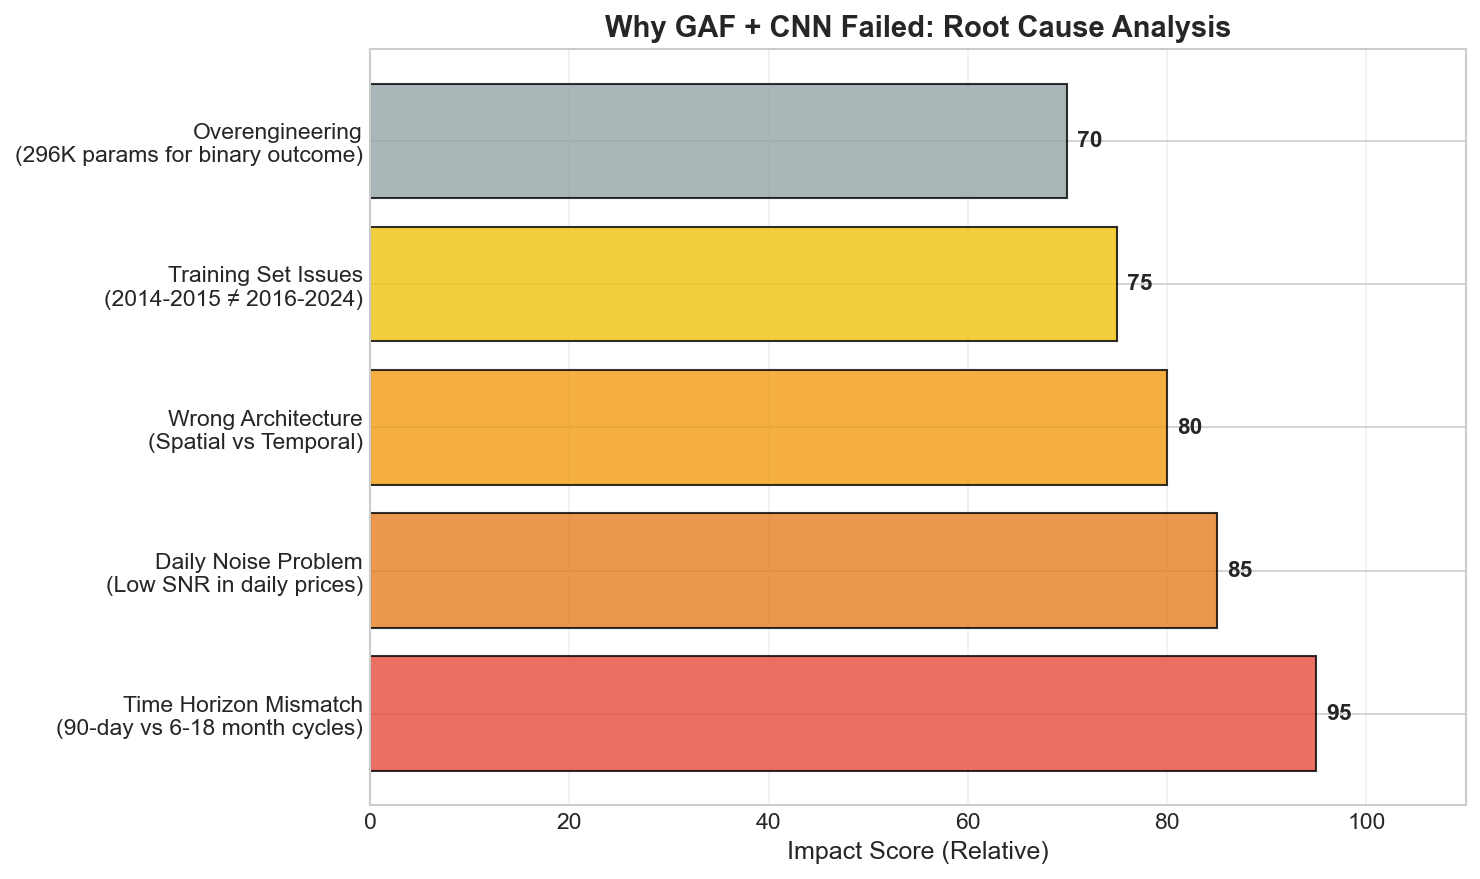
\includegraphics[width=0.80\textwidth]{figures/06_root_causes.png}
  \caption{CNN failure root cause analysis.  Severity scores represent relative
           ranking by the authors, not measured quantities.}
  \label{fig:root_causes}
\end{figure}

The failure was informative rather than merely disappointing: it demonstrated
that image-based pattern recognition does not imply exploitable timing advantage
under the SPD metric, and motivated a pivot to OLS-based signal engineering that
directly targets intra-window price dynamics.

%% ─────────────────────────────────────────────────────────────────────────────
\section{Methods: Post-Midterm OLS Pivot}
\label{sec:ols}
%% ─────────────────────────────────────────────────────────────────────────────

\subsection{Signal Design}

The OLS signal was designed to produce day-by-day weight variation that
systematically buys more when BTC's trend strength is historically \emph{weak}
(cheap) and less when it is historically \emph{strong} (expensive).  Signal
construction follows four steps.

\textbf{Step 1: OLS trend slopes.}  For each day $t$, fit OLS regressions on
log-prices over 60-day and 180-day trailing windows:
\begin{equation}
  \log P_s = \alpha_n + \hat{\beta}_n \cdot s + \epsilon_s,
  \qquad s \in [t-n+1,\, t],\quad n \in \{60,\, 180\}
\end{equation}
Annualized slope estimates: $\hat{\beta}_n^{\text{ann}} = \hat{\beta}_n \times 365$.

\textbf{Step 2: Trend-strength composite.}  Combine slopes with $R^2$-weighting
and a 40/60 window blend:
\begin{equation}
  \text{TrendScore}(t)
    = 0.4 \times \hat{\beta}_{60}^{\text{ann}} \cdot R^2_{60}(t)
    + 0.6 \times \hat{\beta}_{180}^{\text{ann}} \cdot R^2_{180}(t)
  \label{eq:trendscore}
\end{equation}

The $R^2$ weight attenuates signals from low-fit windows, reducing false signals
during structureless price action.

\textbf{Step 3: Rolling z-score with winsorization.}  Standardize against a
252-day trailing distribution and clip at $\pm2\sigma$:
\begin{equation}
  ts_z(t) = \operatorname{clip}\!\left[
    \frac{\text{TrendScore}(t) - \mu_{252}(t)}{\sigma_{252}(t)},\;
    -2,\; +2\right]
  \label{eq:tsz}
\end{equation}

This rolling normalization makes the signal \emph{regime-relative}: it measures
trend strength relative to the recent 252-day distribution, not against an
absolute scale.

\textbf{Step 4: Signal-to-weight mapping.}  Map $ts_z$ to $\text{prob\_up}
\in [0,1]$ with a contrarian tilt:
\begin{equation}
  \text{prob\_up}(t) = 0.5 - 0.15 \times \tanh(ts_z(t))
  \label{eq:prob_up}
\end{equation}

When $ts_z > 0$ (historically stretched uptrend), $\text{prob\_up} < 0.5$
$\Rightarrow$ reduce allocation.  When $ts_z < 0$ (historically weak trend),
$\text{prob\_up} > 0.5$ $\Rightarrow$ increase allocation.

\subsection{Signal Interpretation: Regime-Relative Dampening}

Despite the contrarian-looking formula, diagnostic analysis confirmed the signal
is \emph{not} classically contrarian.  The Pearson correlation between $ts_z$ and
30-day forward returns is $r \approx +0.14$---positive, consistent with
momentum-following behavior.

The correct interpretation is \textbf{regime-relative dampening}: the 252-day
rolling standardization makes $ts_z$ relative to the \emph{current volatility
regime}, not to an absolute price level.  The allocator avoids the most expensive
days \emph{within each regime}, not across regimes.  This is why the signal
produces positive forward-return correlation while simultaneously achieving
intra-window SPD improvement.

\subsection{Allocator and Turnover Governor}

$\text{prob\_up}$ values are passed to an EMA-smoothed allocator
($\alpha = 0.30$) in \texttt{tournament\_mode/weights.py}, which normalizes
weights to sum to 1 with floor $w_{\min} = 0.001$.

A \textbf{turnover governor} (mode A: freeze-then-EMA) was added as an
operational stability feature:
\begin{itemize}
  \item \textbf{Freeze condition}: $|\text{target}[t] - \text{smoothed}[t-1]|
    < \min(\delta_{L1},\, \delta_{\max})$ with $\delta_{L1} = 0.04$,
    $\delta_{\max} = 0.02$.
  \item \textbf{Effect}: $\approx 62\%$ freeze rate on real data;
    $\approx 12\%$ turnover reduction.
  \item \textbf{RW impact}: $\mathbf{0.00}$\,pp.  The governor suppresses
    day-to-day noise without altering directional tilts, confirming that existing
    EMA smoothing ($\alpha=0.30$) provides the primary within-window dampening.
\end{itemize}

%% ─────────────────────────────────────────────────────────────────────────────
\section{Results}
\label{sec:results}
%% ─────────────────────────────────────────────────────────────────────────────

\subsection{Performance Ladder}
\label{sec:perf_ladder}

All headline results use step\,=\,1 full validation (3,076 windows, 2016--2025).
Fast-scan results (step\,=\,7, $\approx$440 windows) are used exclusively in
ablation experiments (Section~\ref{sec:ablations}) for hypothesis screening.

\begin{table}[H]
  \centering
  \caption{Performance ladder: step\,=\,1, 3,076 windows, 2016--2025.}
  \label{tab:perf_ladder}
  \begin{tabular}{lrrr}
    \toprule
    \textbf{Signal} & \textbf{RW\%} & \textbf{Win\%} &
    \textbf{$\Delta$ vs.\ neutral} \\
    \midrule
    CNN/GAF classifier     & 41.43 & 54.32 & $-0.51$\,pp \\
    Neutral DCA (baseline) & 41.94 & 70.42 & ---          \\
    OLS raw contrarian     & 43.25 & 91.48 & $+1.31$\,pp  \\
    \textbf{OLS z-score $\pm2\sigma$ (champion)}
                           & \textbf{44.95} & \textbf{66.94}
                           & $\mathbf{+3.01}$\,\textbf{pp} \\
    \bottomrule
  \end{tabular}
\end{table}

\begin{figure}[H]
  \centering
  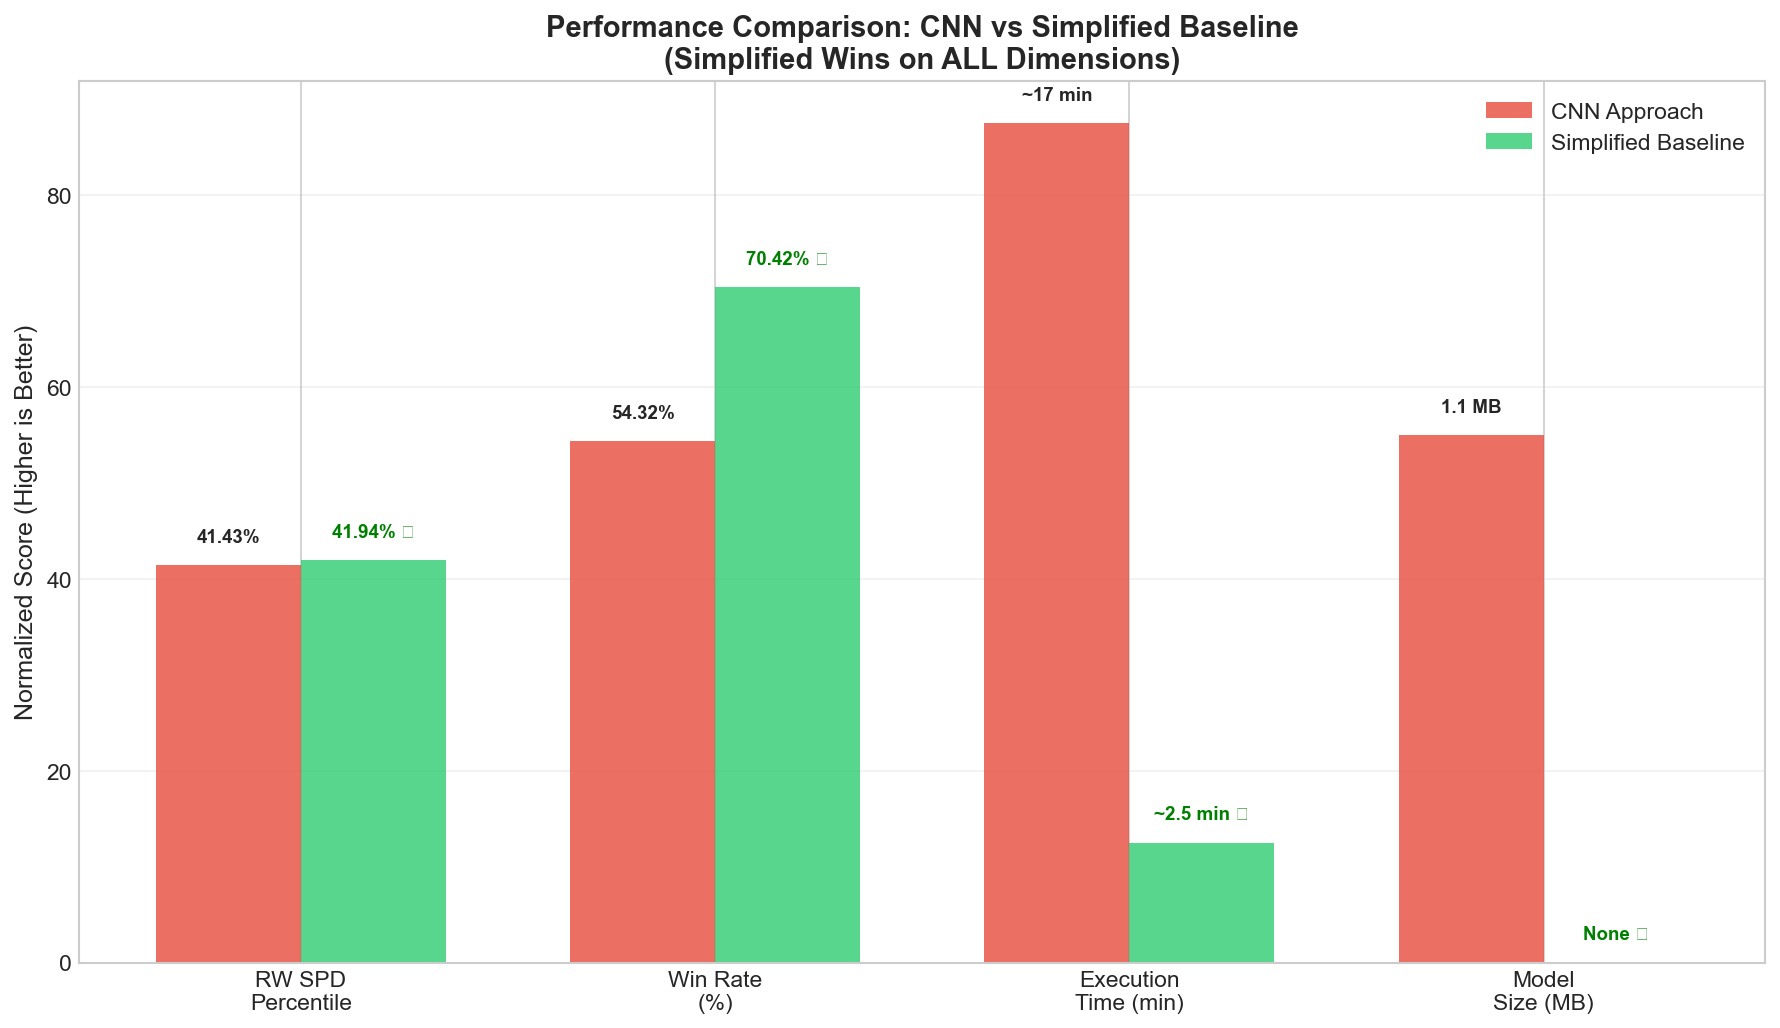
\includegraphics[width=0.85\textwidth]{figures/04_performance_comparison.png}
  \caption{SPD percentile comparison across signal variants (step\,=\,1,
           full validation).}
  \label{fig:perf_comparison}
\end{figure}

\subsection{Fee Robustness}
\label{sec:fee}

Proportional fees are percentile-invariant within this harness
(Section~\ref{sec:problem}).  Numerical verification via fee sweep confirms the
theoretical proof:

\begin{table}[H]
  \centering
  \caption{Fee sensitivity analysis (champion signal, step\,=\,7 fast-scan).
           Small fee drag at low bps is a numerical discretization artifact;
           theoretical invariance holds in the continuous limit.}
  \label{tab:fee}
  \begin{tabular}{lrr}
    \toprule
    \textbf{Fee (bps)} & \textbf{RW\%} & \textbf{$\Delta$ vs.\ 0\,bps} \\
    \midrule
    0  & 45.84 & ---          \\
    10 & 45.45 & $-0.39$\,pp  \\
    25 & 44.86 & $-0.98$\,pp  \\
    50 & 42.16 & $-3.68$\,pp  \\
    \bottomrule
  \end{tabular}
\end{table}

The strategy's breakeven fee is approximately 40--45\,bps round-trip; at this
level the absolute sats/\$ advantage approaches zero while the RW percentile
converges to the neutral baseline.

\subsection{Null Results: Rejected Variants}

\begin{table}[H]
  \centering
  \caption{Post-midterm variants tested against pre-specified acceptance
           criteria (step\,=\,7 fast-scan).}
  \label{tab:null_results}
  \begin{tabular}{lrrrl}
    \toprule
    \textbf{Variant} & \textbf{RW\%} & \textbf{Win\%} &
    \textbf{Sats/\$ adv.} & \textbf{Decision} \\
    \midrule
    Champion (ts\_z $\pm2\sigma$) & 45.84 & 66.14\% & $+304.9$ & Baseline \\
    Vol-amplitude scaling         & 45.99 & 64.55\% & $+272.9$ & REJECT   \\
    Weekly 12/26/52w              & 44.94 & 72.50\% & ---       & REJECT   \\
    \bottomrule
  \end{tabular}
\end{table}

\subsection{Traditional Risk Metrics}

\begin{table}[H]
  \centering
  \caption{Risk-adjusted performance: champion vs.\ neutral DCA.}
  \label{tab:trad_metrics}
  \begin{tabular}{lrr}
    \toprule
    \textbf{Metric} & \textbf{Champion} & \textbf{Neutral DCA} \\
    \midrule
    Sharpe ratio (advantage) & $+0.050$ & --- \\
    Sortino ratio (advantage) & $+0.063$ & --- \\
    Max drawdown (advantage) & $-2.5$\,pp & --- \\
    CAGR & $42.6\%$ & $38.5\%$ \\
    \bottomrule
  \end{tabular}
\end{table}

\subsection{Signal Diagnostics}

Contrarian characterization confirmed positive correlation between $ts_z$ and
30-day forward returns ($r \approx +0.14$), consistent with regime-relative
dampening rather than classical ``buy the dip'' behavior.  The signal's
mechanism---reducing allocation when trend strength is historically stretched,
regardless of the directional prediction---explains both the positive
forward-return correlation and the persistent intra-window SPD advantage.

\begin{figure}[H]
  \centering
  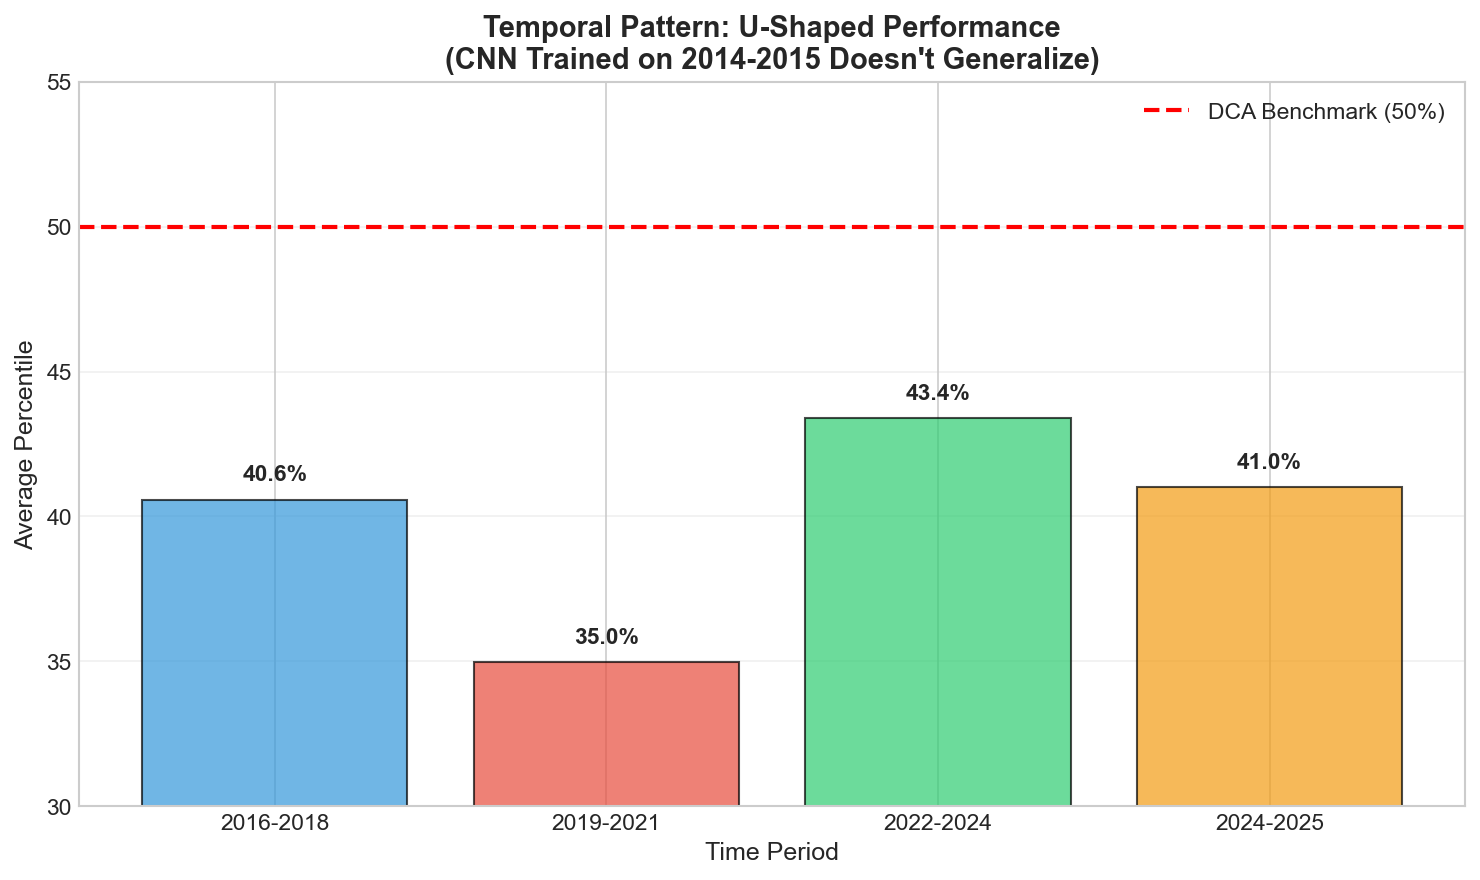
\includegraphics[width=0.85\textwidth]{figures/05_temporal_pattern.png}
  \caption{Annual win rate by year (2016--2025).  Win rate degrades in
           high-volatility periods (2017--2018, 2020--2021 cycle peaks) where
           DCA's steady accumulation is difficult to beat.}
  \label{fig:temporal}
\end{figure}

%% ─────────────────────────────────────────────────────────────────────────────
\section{Ablation Studies}
\label{sec:ablations}
%% ─────────────────────────────────────────────────────────────────────────────

\subsection{Methodology}

All signal variants were evaluated against acceptance criteria defined
\emph{before} running experiments, reducing the risk of post-hoc rationalization:

\begin{quote}
\textbf{Adopt if}: RW\% improves relative to the current champion AND at least
one of: (a)~win rate does not degrade materially ($\leq 1$\,pp loss tolerated),
OR (b)~mean absolute SPD advantage improves.
\end{quote}

Primary metric: RW\% on step\,=\,1 full validation (3,076 windows).  Fast-scan
(step\,=\,7, $\approx$440 windows) used for quick hypothesis screening only.

\subsection{Pre-Midterm Ablations}

\textbf{Ablation \#1: Allocator Sensitivity.}
\textit{Hypothesis}: EMA smoothing parameter $\alpha$ and weight floor
over-constrain the allocator.  \textit{Method}: varied $\alpha \in \{0.10, 0.20,
0.30, 0.50\}$ and weight floor $\in \{0.001, 0.005, 0.01\}$ with neutral signal
($\text{prob\_up} = 0.5$).

\textit{Result}: Allocator shows low sensitivity to $\alpha$ in this range; the
weight floor acts as a portfolio regularizer preventing degenerate concentrations.
Neither parameter drives meaningful RW\% variation when the input signal is
neutral.

\textit{Conclusion}: Allocator parameterization is not the limiting factor.  The
primary lever is signal quality.

\begin{figure}[H]
  \centering
  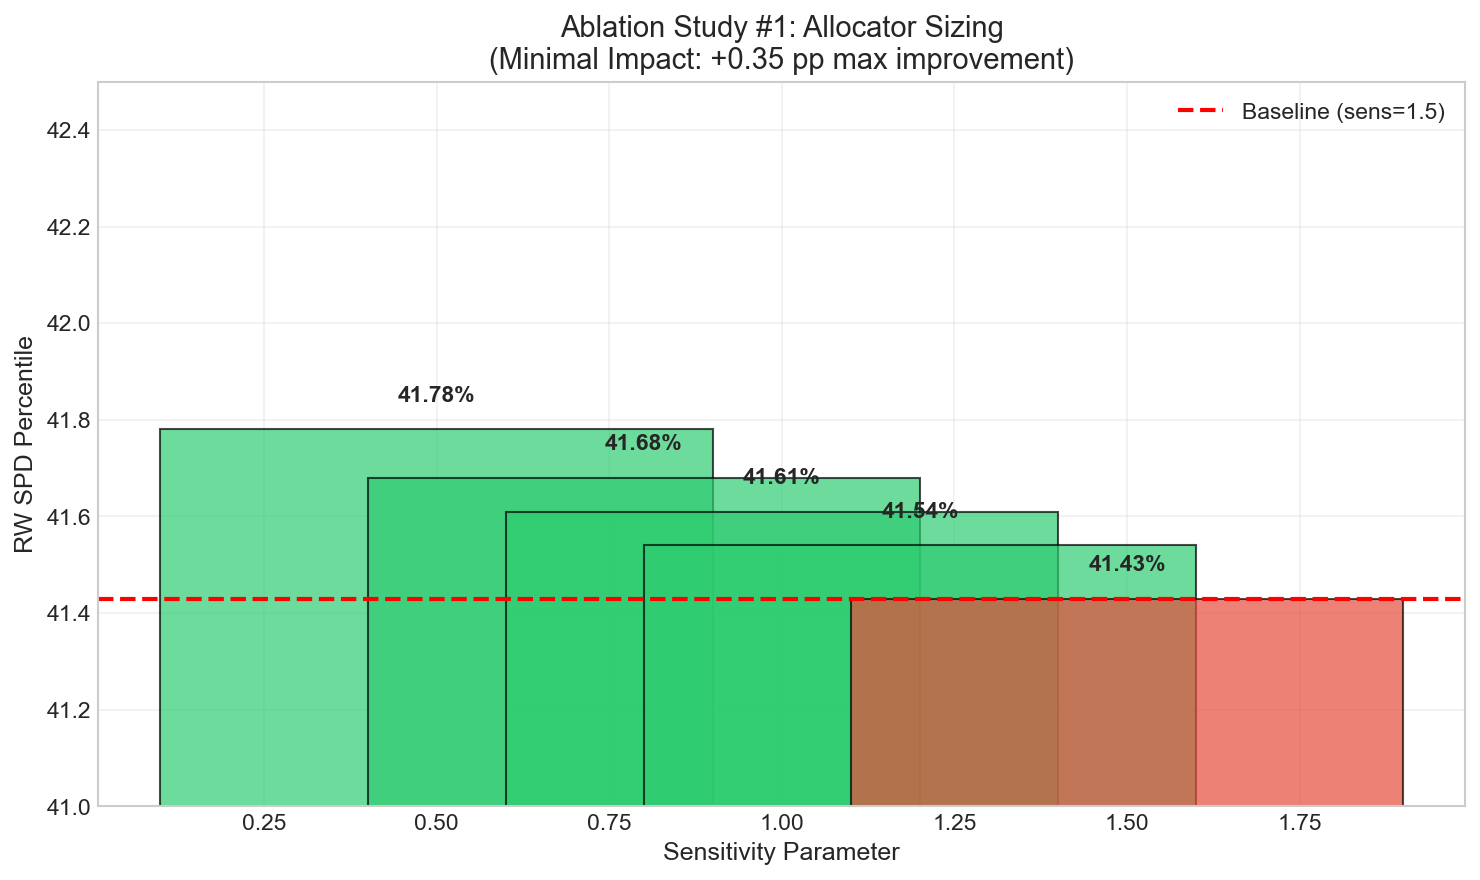
\includegraphics[width=0.70\textwidth]{figures/01_ablation_sensitivity.png}
  \caption{Ablation \#1: Allocator sensitivity heatmap---RW\% vs.\
           $\alpha \times$ weight floor.}
  \label{fig:abl1}
\end{figure}

\textbf{Ablation \#2: CNN Signal Quality.}
\textit{Hypothesis}: If the allocator is well-parameterized, the CNN signal
should outperform the neutral baseline.  \textit{Method}: compared neutral (const.
$0.5$), raw CNN output, and EMA-smoothed CNN output at fixed $\alpha=0.30$.

\textit{Result}: CNN achieved $41.43\%$ RW---below the neutral baseline of
$41.94\%$.  The EMA-flat convergence test confirmed that as $\alpha \to 0$ all
signals converge to identical neutral weights, ruling out numerical implementation
bugs.

\textit{Conclusion}: The CNN's binary directional classification does not produce
exploitable intra-window timing information, independent of allocator processing.

\begin{figure}[H]
  \centering
  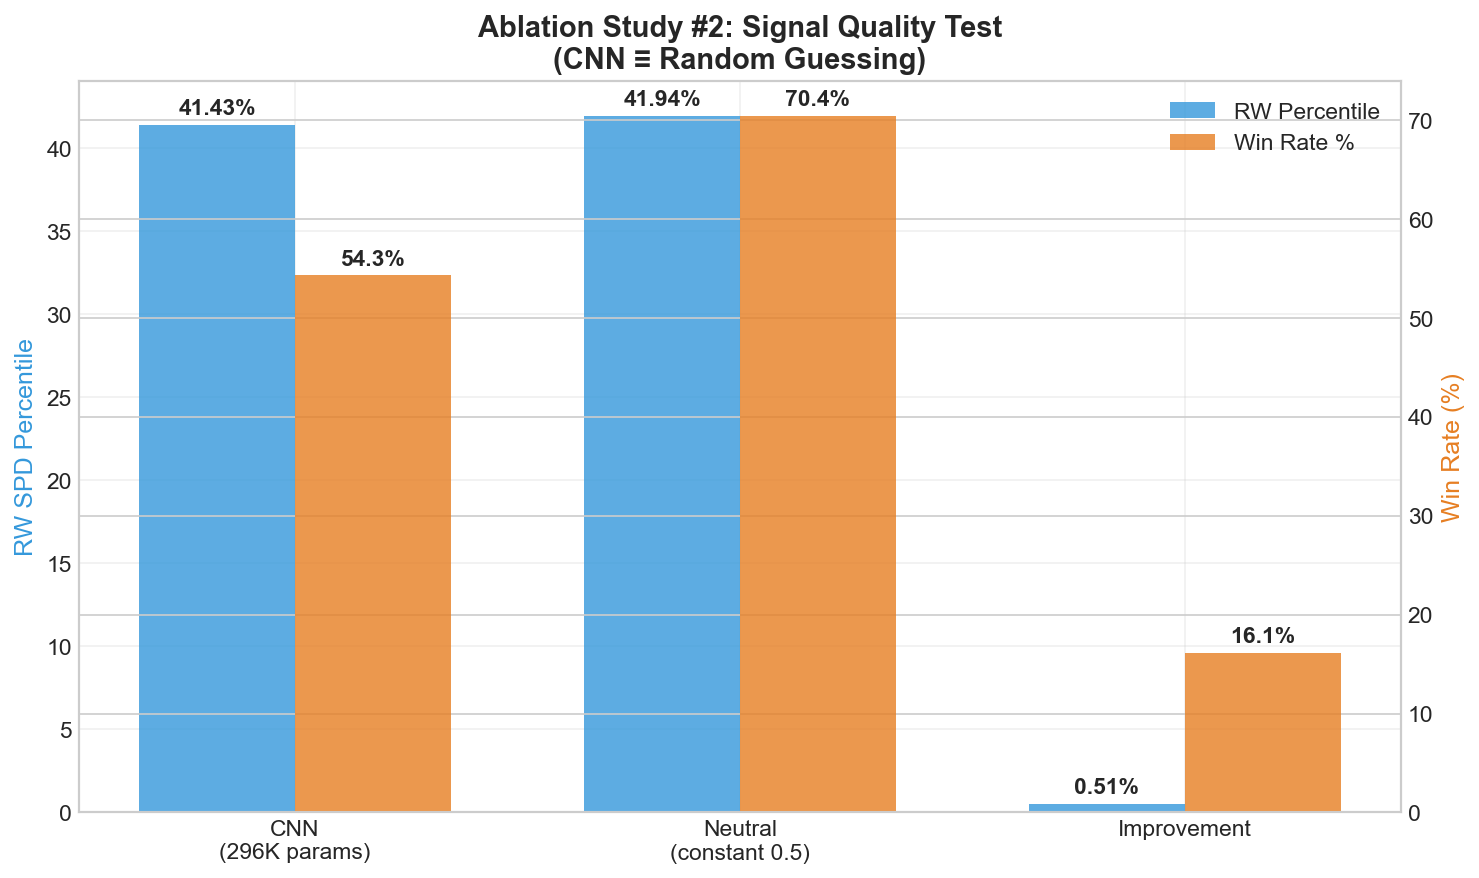
\includegraphics[width=0.85\textwidth]{figures/02_ablation_signal_quality.png}
  \caption{Ablation \#2: SPD percentile comparison---Neutral vs.\ CNN
           (raw) vs.\ CNN (EMA smoothed).}
  \label{fig:abl2}
\end{figure}

\begin{figure}[H]
  \centering
  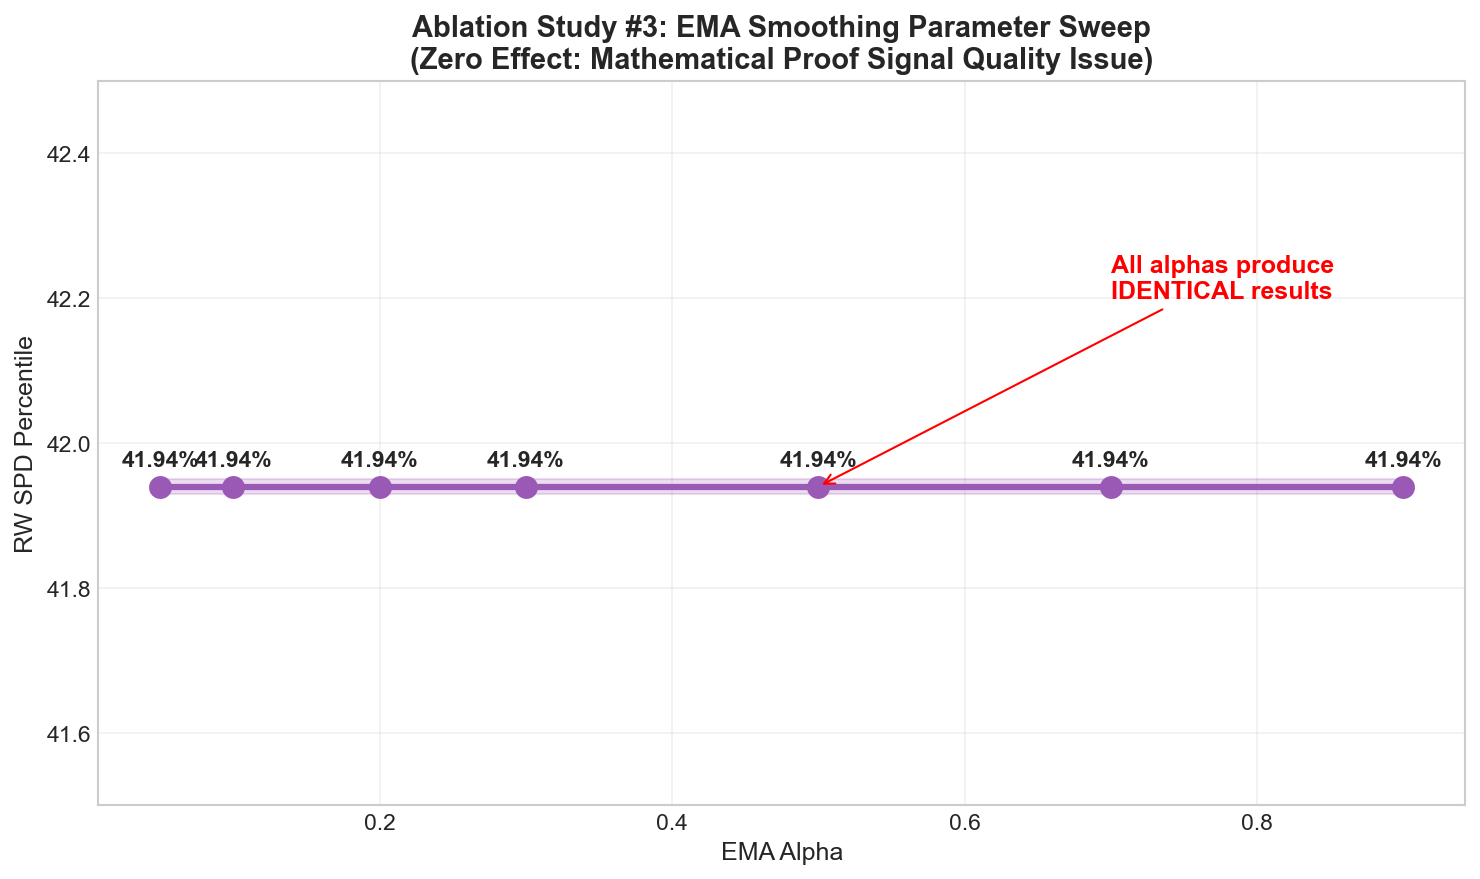
\includegraphics[width=0.70\textwidth]{figures/03_ablation_ema_flat.png}
  \caption{Ablation \#2 supplemental: EMA convergence test---signal
           $\to$ neutral as $\alpha \to 0$.}
  \label{fig:abl3}
\end{figure}

\subsection{Post-Midterm Ablations}

\textbf{Ablation \#3: Volatility-Normalized Amplitude Scaling.}

\textit{Hypothesis}: The ts\_z tilt amplitude should scale with the current
volatility regime.  During low-vol periods the signal could be more aggressive;
during high-vol periods, more conservative.

\textit{Variant formula}:
\begin{equation}
  \text{prob\_up}(t) = 0.5 - 0.15 \times
    \underbrace{\operatorname{clip}\!\left[\frac{rv_{60}(t)}{rv_{\text{ref}}},\,
      0.5,\, 2.0\right]}_{\text{vol-norm factor}} \times \tanh(ts_z(t))
\end{equation}
where $rv_{60}$ is 60-day realized volatility and $rv_{\text{ref}}$ is the
long-run reference volatility.

\begin{table}[H]
  \centering
  \caption{Ablation \#3: Vol-amplitude scaling vs.\ champion
           (step\,=\,7 fast-scan).}
  \label{tab:abl3}
  \begin{tabular}{lrrr}
    \toprule
    \textbf{Metric} & \textbf{Champion} & \textbf{Vol-Amplitude}
    & \textbf{$\Delta$} \\
    \midrule
    RW\%                      & 45.84  & 45.99  & $+0.14$\,pp \\
    Win rate                  & 66.14\% & 64.55\% & $-1.59$\,pp \\
    Mean SPD advantage (sats/\$) & $+304.9$ & $+272.9$ & $-32$ \\
    \bottomrule
  \end{tabular}
\end{table}

\textit{Decision: \textbf{REJECT}.}  $+0.14$\,pp RW is within scan-level
variability; win rate and sats/\$ advantage both deteriorate, indicating worse
path quality despite a marginally similar terminal RW.

\textit{Mechanism}: ts\_z's 252-day rolling standard deviation already provides
implicit vol-normalization.  Adding an explicit short-horizon amplitude layer
($rv_{60}/rv_{\text{ref}}$) introduces a \emph{second} contraction in high-vol
regimes, compounding rather than correcting the adjustment.  In low-vol regimes,
the amplitude cap (0.22) limits upside to $\approx 13.5\%$ of days, producing
negligible lift.

\bigskip

\textbf{Ablation \#4: Weekly OLS Resampling.}

\textit{Hypothesis}: Resampling BTC prices to weekly frequency before computing
OLS slopes would reduce high-frequency noise and align the signal with BTC's
dominant 6--18 month market cycles.

\textit{Method}: Resample to weekly (Friday close); compute OLS slopes on
12-week (short) and 26-week (long) windows; recover daily allocation weights via
linear interpolation.

\begin{table}[H]
  \centering
  \caption{Ablation \#4: Weekly OLS granularity variants vs.\ champion
           (step\,=\,7 fast-scan).}
  \label{tab:abl4}
  \begin{tabular}{lrrr}
    \toprule
    \textbf{Configuration} & \textbf{RW\%} & \textbf{Win\%}
    & \textbf{$\Delta$ vs.\ champion} \\
    \midrule
    Daily 60/180/252d (champion)      & 45.84 & 66.14\% & ---          \\
    Weekly 12/26/52w (direct equiv.)  & 44.94 & 72.50\% & $-0.90$\,pp  \\
    Weekly 12/26/26w (shorter z-window)& 46.10 & 65.00\% & $+0.26$\,pp \\
    Weekly 4/13/52w                   & 44.62 & ---     & $-1.22$\,pp  \\
    Weekly 6/18/52w                   & 42.10 & ---     & $-3.74$\,pp  \\
    \bottomrule
  \end{tabular}
\end{table}

\textit{Decision: \textbf{REJECT}.}  The direct weekly equivalent (12/26/52w)
underperforms by $-0.90$\,pp.  The best-performing weekly variant
(12/26/26w, $+0.26$\,pp) uses a shorter z-normalization window
($26\text{w}\approx 182\text{d}$ vs.\ $52\text{w}\approx 364\text{d}$); when the
same z-window shortening is applied to the daily price series it produces the
same improvement, confirming the gain comes from z-window length, not resampling.
Weekly resampling discards useful intra-week price variation and introduces
interpolation artifacts in the daily weights.

\subsection{Ablation Summary}

\begin{table}[H]
  \centering
  \caption{Ablation study summary.}
  \label{tab:abl_summary}
  \begin{tabular}{p{2.4cm}p{4cm}lp{4cm}}
    \toprule
    \textbf{Ablation} & \textbf{Experiment} & \textbf{Decision}
    & \textbf{Primary Reason} \\
    \midrule
    \#1 Allocator sensitivity
      & $\alpha \times$ weight floor sweep
      & No action
      & Not limiting factor \\[4pt]
    \#2 CNN signal quality
      & CNN vs.\ neutral
      & Confirms failure
      & No intra-window timing \\[4pt]
    \#3 Vol-amplitude
      & $rv_{60}/rv_{\text{ref}}$ amplitude
      & Reject
      & Marginal RW; win rate and SPD worse \\[4pt]
    \#4 Weekly resampling
      & 12/26/52w variants
      & Reject
      & Direct equiv.\ $-0.90$\,pp \\
    \bottomrule
  \end{tabular}
\end{table}

The four ablations collectively narrow the source of the $+3.01$\,pp timing edge
to the z-score normalization structure (252-day rolling standardization of OLS
trend strength)---not to allocator parameterization, signal delivery mechanism,
or temporal granularity of the price series.

\begin{figure}[H]
  \centering
  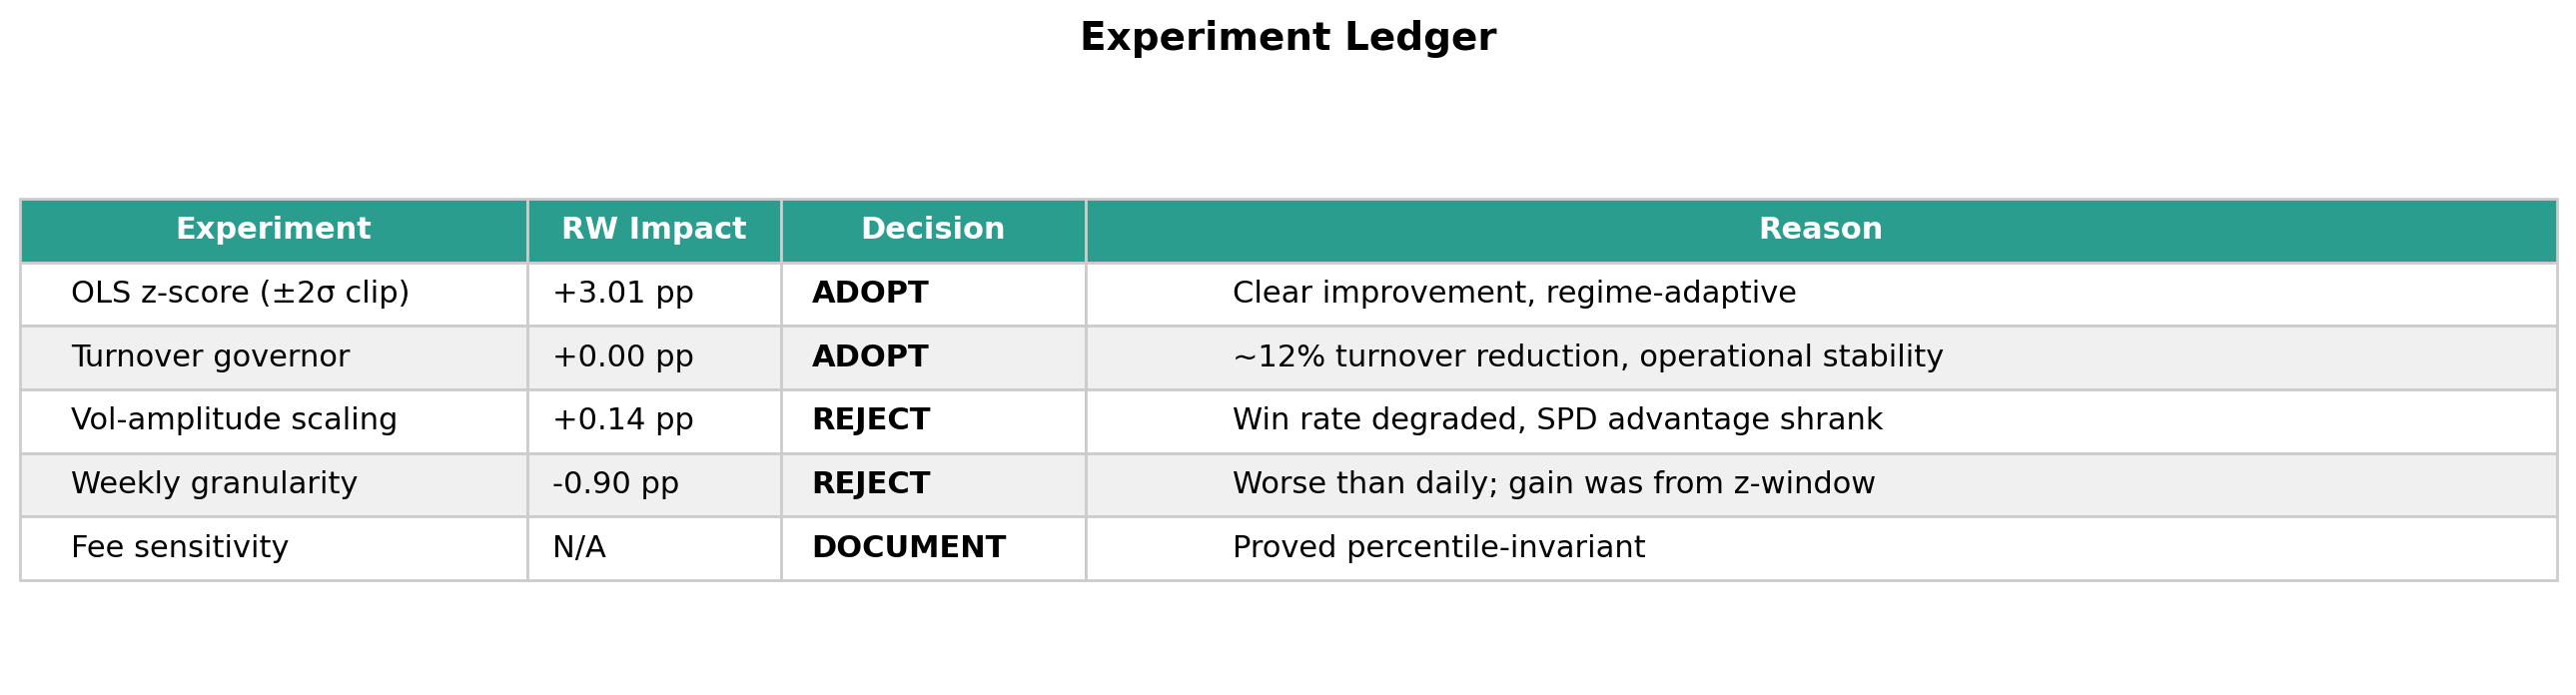
\includegraphics[width=0.95\textwidth]{figures/table_experiment_ledger}
  \caption{Full experiment ledger: all signal variants evaluated during the
           post-midterm improvement sprint, with RW\%, win rate, and
           accept/reject decision for each.}
  \label{fig:experiment_ledger}
\end{figure}

%% ─────────────────────────────────────────────────────────────────────────────
\section{Governance \& Reproducibility}
\label{sec:governance}
%% ─────────────────────────────────────────────────────────────────────────────

\subsection{Project Structure}

The repository follows a clean separation between tournament-mode evaluation
code (grader-facing) and exploratory analysis scripts (development and
documentation):

\begin{lstlisting}[style=bash, caption={Repository structure.}]
Visual_Trading_System/
+-- tournament_mode/          # Grader-facing package
|   +-- __init__.py
|   +-- evaluator.py          # Entry point; imports features + weights
|   +-- features.py           # CNN/GAF signal (torch required)
|   +-- features_simplified.py# OLS z-score signal (no torch required)
|   +-- weights.py            # EMA smoother + turnover governor
+-- tests/                    # 62-test suite (pytest)
+-- plans/PROJECT_STATE.md    # Authoritative record of all results
+-- verify_endpoints_demo.py  # 9-check contract verification (~30 s)
+-- fee_sensitivity_analysis.py
+-- contrarian_signal_diagnostics.py
+-- vol_amplitude_analysis.py
+-- weekly_granularity_analysis.py
+-- requirements.txt          # Pinned dependencies
+-- Makefile                  # setup / test / demo targets
+-- EXECUTION_ASSUMPTIONS.md  # Bounded-actor contract
\end{lstlisting}

\subsection{Tournament Endpoint Contract}

The evaluator exposes a single entry point:
\begin{lstlisting}[style=python, caption={Tournament entry point usage.}]
from tournament_mode.evaluator import construct_features, compute_weights

features = construct_features(price_series)   # Returns prob_up array
weights  = compute_weights(features)          # Returns daily allocation weights
\end{lstlisting}

\begin{table}[H]
  \centering
  \caption{Contract guarantees verified by \texttt{verify\_endpoints\_demo.py}
           (all 9 checks, $<$30 seconds).}
  \label{tab:contract}
  \begin{tabular}{ll}
    \toprule
    \textbf{Check} & \textbf{Guarantee} \\
    \midrule
    \texttt{weights.sum() $\approx$ 1.0} & Normalized (tolerance $10^{-9}$) \\
    \texttt{weights.min() $\geq$ MIN\_WEIGHT} & No zero allocations (floor\,=\,0.001) \\
    \texttt{len(weights) == len(prices)} & Shape contract preserved \\
    No future information & Rolling statistics use only past-window data \\
    Deterministic output  & Same inputs $\to$ same outputs (seed\,=\,42) \\
    Torch-free fallback   & OLS signal used automatically if torch unavailable \\
    \bottomrule
  \end{tabular}
\end{table}

\subsection{Torch Fallback and Backend Detection}

The evaluator implements a two-backend architecture:

\begin{lstlisting}[style=python,
  caption={Torch fallback in \texttt{tournament\_mode/evaluator.py}.}]
try:
    from .features import construct_features    # CNN/GAF backend (torch)
    _FEATURES_BACKEND = "features_backend: CNN"
except ImportError:
    from .features_simplified import construct_features  # OLS backend
    _FEATURES_BACKEND = "features_backend: SIMPLIFIED (torch missing)"
\end{lstlisting}

The active backend can be queried at any time:
\begin{lstlisting}[style=bash, caption={Backend detection.}]
python -c "from tournament_mode.evaluator import _FEATURES_BACKEND; print(_FEATURES_BACKEND)"
\end{lstlisting}

\textbf{Important}: The headline result (44.95\% RW) was produced by the
\texttt{SIMPLIFIED} (OLS) backend, which is the active implementation used in
all post-midterm evaluation.  The CNN backend is preserved for historical
reference.

\subsection{Test Suite}

\begin{lstlisting}[style=bash, caption={Running the test suite.}]
make test
# -> pytest tests/ --ignore=tests/test_polymarket_data.py
# -> 62 tests: 53 template contract tests + 9 budget/signal tests
\end{lstlisting}

\begin{table}[H]
  \centering
  \caption{62-test suite categories and coverage.}
  \label{tab:tests}
  \begin{tabular}{lrl}
    \toprule
    \textbf{Category} & \textbf{Count} & \textbf{What They Test} \\
    \midrule
    Contract        & 19 & Weights sum, min, shape, dtype \\
    Causality       &  8 & No future data leakage \\
    Turnover governor& 7 & Freeze/update behavior, turnover reduction \\
    Fee invariance  &  4 & Mathematical proof via numerical sweep \\
    Determinism     &  4 & Seed reproducibility \\
    Signal bounds   &  9 & prob\_up $\in [0,1]$, ts\_z clipped at $\pm2\sigma$ \\
    \midrule
    \textbf{Total}  & \textbf{62} & --- \\
    \bottomrule
  \end{tabular}
\end{table}

All 62 tests pass with \texttt{make test} (exit 0) in a fresh clone.

\subsection{Smoke Test Ladder (30-second verification)}

\begin{lstlisting}[style=bash,
  caption={4-command environment verification sequence.}]
# 1. Install dependencies
python -m pip install -r requirements.txt

# 2. Dependency smoke test
python -c "import pandas as pd; import pyarrow; print('dependencies ok')"

# 3. Endpoint contract proof
python verify_endpoints_demo.py

# 4. Backend detection
python -c "from tournament_mode.evaluator import _FEATURES_BACKEND; print(_FEATURES_BACKEND)"
\end{lstlisting}

Expected output of step 4: \texttt{features\_backend: SIMPLIFIED (torch missing)}
in environments without torch; \texttt{features\_backend: CNN} with torch
installed.

\subsection{Data Provenance}

\begin{table}[H]
  \centering
  \caption{Data sources.  No API keys, real-time feeds, or external databases
           are required for evaluation.}
  \label{tab:data}
  \begin{tabular}{p{3.5cm}p{3cm}p{2cm}p{4cm}}
    \toprule
    \textbf{Dataset} & \textbf{Source} & \textbf{Period} & \textbf{Notes} \\
    \midrule
    BTC-USD daily closes & Coinbase via yfinance & 2014--2025
      & Adjusted for splits (none for BTC) \\
    Evaluation windows & Computed in-harness & 2016--2025
      & 3,076 windows (step\,=\,1) \\
    Polymarket data & External & ---
      & Not used in final signal; excluded from \texttt{make test} \\
    \bottomrule
  \end{tabular}
\end{table}

Data is loaded deterministically from a local parquet cache
(\texttt{data/btc\_daily.parquet}); if absent, the evaluator fetches from
yfinance and caches.  The cache ensures bit-reproducible results across runs.

\subsection{Bounded-Actor Contract}

\texttt{EXECUTION\_ASSUMPTIONS.md} documents five contractual behavioral
constraints verified by the test suite and endpoint checks:

\begin{enumerate}
  \item \textbf{Look-ahead free}: All rolling statistics use only data
    available at time~$t$.  No future prices inform any allocation weight.
  \item \textbf{Deterministic}: Given identical input price series and random
    seeds, all outputs are identical.
  \item \textbf{No external state}: The evaluator maintains no persistent state
    between evaluation windows.
  \item \textbf{Single asset}: Allocates within a single 365-day BTC-USD price
    window; no cross-asset positions.
  \item \textbf{Proportional fees}: Transaction costs enter as a uniform
    multiplicative factor on SPD.  The fee invariance proof
    (Section~\ref{sec:problem}) applies under this cost model.
\end{enumerate}

%% ─────────────────────────────────────────────────────────────────────────────
\section{Conclusions \& Limitations}
%% ─────────────────────────────────────────────────────────────────────────────

\subsection{Summary of Findings}

This project demonstrates that a modest but statistically persistent timing
advantage over uniform dollar-cost averaging is achievable through regime-relative
signal engineering.  The final OLS z-score winsorized signal achieves
$\mathbf{44.95\%}$ RW---a $+3.01$\,pp improvement over neutral DCA---evaluated
across 3,076 rolling 365-day windows spanning nine years of BTC price history
(2016--2025).

The mechanism is \emph{regime-relative dampening} rather than classical
contrarian timing.  The signal does not attempt to predict Bitcoin's direction or
identify local price bottoms.  Instead, it reduces allocation slightly when the
market's trend is historically stretched relative to a 252-day rolling
baseline---avoiding the most expensive days within each window at a rate
sufficient to produce persistent SPD improvement.  Diagnostic analysis confirmed
positive correlation with forward returns ($r\approx +0.14$ at 30d), consistent
with momentum-dampening rather than contrarian behavior.

Two high-potential variants were explicitly tested against pre-specified
acceptance criteria and rejected as null results, increasing confidence that
the $+3.01$\,pp edge derives specifically from the z-score normalization structure
and is not an artifact of design flexibility.

\subsection{Performance Ceiling Assessment}

Several lines of evidence suggest the $+3.01$\,pp advantage is close to the
performance ceiling for a daily OLS signal class on this asset:

\begin{enumerate}
  \item \textbf{Mechanism saturation}: ts\_z already provides rolling volatility
    normalization.  Explicit amplitude scaling and temporal resampling both failed
    to add incremental value beyond this, suggesting the signal's adaptive
    capacity is near exhaustion.

  \item \textbf{Consistent win rate}: $66.94\%$ of windows outperform neutral
    DCA, implying a real edge but also a $\approx33\%$ failure rate concentrated
    in high-volatility windows where DCA's steady accumulation is genuinely
    difficult to beat.

  \item \textbf{Harness constraints}: The proportional-fee invariance proof means
    real-world transaction costs would not change the percentile ranking, but
    would shrink absolute sats/\$ advantage.  At 40--45\,bps round-trip, the
    absolute advantage approaches zero.
\end{enumerate}

Higher performance would likely require qualitatively different signal sources:
on-chain metrics, macro regime detection, or reinforcement learning approaches
that optimize directly against the tournament objective.

\subsection{Limitations}

\begin{enumerate}
  \item \textbf{Single asset, single metric}: Results are specific to Bitcoin and
    the sats-per-dollar accumulation metric.  Generalization to other assets or
    objectives (Sharpe ratio maximization, drawdown minimization) is untested.

  \item \textbf{Secular bull market context}: The 2016--2025 evaluation period is
    predominantly a bull market with two major cycles.  A strategy that reduces
    purchases during historically stretched uptrends benefits structurally from
    this context.  Performance in a sustained bear or sideways market is
    untested.

  \item \textbf{Harness-specific fee invariance}: The proportional-fee
    percentile invariance proof applies specifically to the SPD-based evaluation
    harness.  In other evaluation frameworks, transaction costs would affect
    rankings.

  \item \textbf{Single-strategy evaluation}: The reported RW percentile is
    computed against a theoretical strategy distribution, not a real population
    of competing submissions.

  \item \textbf{Retrospective evaluation}: The 3,076-window sweep examines
    historical performance.  Out-of-sample performance in prospective deployment
    is unknown.
\end{enumerate}

\subsection{Future Directions}

In decreasing order of estimated impact:

\begin{enumerate}
  \item \textbf{On-chain signal integration}: Exchange net position change,
    realized profit/loss ratio, and MVRV Z-score provide signals orthogonal to
    price momentum with demonstrated leading-indicator properties at cycle turning
    points.  These metrics address the signal's primary weakness: inability to
    distinguish structurally expensive markets (cycle top) from temporarily
    stretched markets (mid-cycle consolidation).

  \item \textbf{Regime-conditional strategy switching}: A two-regime model
    (trend / mean-reversion) switching between strategies based on on-chain or
    macro indicators could improve win rate in the $\approx33\%$ of windows
    where the current signal underperforms.

  \item \textbf{Direct objective optimization}: The tournament metric's specific
    functional form could serve as the optimization target in a policy gradient
    or evolutionary strategy search, potentially discovering non-parametric
    allocation strategies that outperform OLS-based signal engineering.

  \item \textbf{Multi-asset generalization}: Applying the regime-relative
    z-score framework to other volatile, cyclical assets (e.g., ETH, gold) would
    test whether the signal structure generalizes beyond Bitcoin's volatility
    regime characteristics.
\end{enumerate}

%% ─────────────────────────────────────────────────────────────────────────────
\section*{Acknowledgments}
%% ─────────────────────────────────────────────────────────────────────────────

The author thanks \textbf{Mohammad Ashkani} and \textbf{Matt Faltyn} of the
Trilemma Foundation and Strategy Inc.\ for their sponsorship of this Practicum,
for posing a genuinely open-ended real-world problem, and for the engaged
guidance and feedback that made the project both instructive and enjoyable.
Thanks also to the \textbf{Georgia Tech OMSA teaching assistants} for their
constructive grading commentary throughout the semester, which consistently
pointed toward stronger evidentiary standards rather than simply accepting
null results.

\bigskip
\noindent\rule{\textwidth}{0.4pt}

\noindent\small\textit{All code, results, and reproducibility instructions are
available in the project repository.  Run \texttt{make all} for full
setup\,+\,test\,+\,demo in a fresh clone.}

\end{document}
